\documentclass[10pt,]{article}
\usepackage[left=1in,top=1in,right=1in,bottom=1in]{geometry}
\newcommand*{\authorfont}{\fontfamily{phv}\selectfont}
\usepackage[]{mathpazo}


  \usepackage[T1]{fontenc}
  \usepackage[utf8]{inputenc}




\usepackage{abstract}
\renewcommand{\abstractname}{}    % clear the title
\renewcommand{\absnamepos}{empty} % originally center

\renewenvironment{abstract}
 {{%
    \setlength{\leftmargin}{0mm}
    \setlength{\rightmargin}{\leftmargin}%
  }%
  \relax}
 {\endlist}

\makeatletter
\def\@maketitle{%
  \newpage
%  \null
%  \vskip 2em%
%  \begin{center}%
  \let \footnote \thanks
    {\fontsize{18}{20}\selectfont\raggedright  \setlength{\parindent}{0pt} \@title \par}%
}
%\fi
\makeatother




\setcounter{secnumdepth}{0}

\usepackage{longtable,booktabs}

\usepackage{graphicx,grffile}
\makeatletter
\def\maxwidth{\ifdim\Gin@nat@width>\linewidth\linewidth\else\Gin@nat@width\fi}
\def\maxheight{\ifdim\Gin@nat@height>\textheight\textheight\else\Gin@nat@height\fi}
\makeatother
% Scale images if necessary, so that they will not overflow the page
% margins by default, and it is still possible to overwrite the defaults
% using explicit options in \includegraphics[width, height, ...]{}
\setkeys{Gin}{width=\maxwidth,height=\maxheight,keepaspectratio}


\title{Case study 1: Effect of chemical exposures on preterm birth  }
 



\author{\Large Olivier Binette, Brian Kundinger and Joe
Mathews\vspace{0.05in} \newline\normalsize\emph{}  }


\date{}

\usepackage{titlesec}

\titleformat*{\section}{\normalsize\bfseries}
\titleformat*{\subsection}{\normalsize\itshape}
\titleformat*{\subsubsection}{\normalsize\itshape}
\titleformat*{\paragraph}{\normalsize\itshape}
\titleformat*{\subparagraph}{\normalsize\itshape}


\usepackage{natbib}
\bibliographystyle{plainnat}
\usepackage[strings]{underscore} % protect underscores in most circumstances



\newtheorem{hypothesis}{Hypothesis}
\usepackage{setspace}


% set default figure placement to htbp
\makeatletter
\def\fps@figure{htbp}
\makeatother

\usepackage{hyperref}

% move the hyperref stuff down here, after header-includes, to allow for - \usepackage{hyperref}

\makeatletter
\@ifpackageloaded{hyperref}{}{%
\ifxetex
  \PassOptionsToPackage{hyphens}{url}\usepackage[setpagesize=false, % page size defined by xetex
              unicode=false, % unicode breaks when used with xetex
              xetex]{hyperref}
\else
  \PassOptionsToPackage{hyphens}{url}\usepackage[draft,unicode=true]{hyperref}
\fi
}

\@ifpackageloaded{color}{
    \PassOptionsToPackage{usenames,dvipsnames}{color}
}{%
    \usepackage[usenames,dvipsnames]{color}
}
\makeatother
\hypersetup{breaklinks=true,
            bookmarks=true,
            pdfauthor={Olivier Binette, Brian Kundinger and Joe
Mathews ()},
             pdfkeywords = {},  
            pdftitle={Case study 1: Effect of chemical exposures on
preterm birth},
            colorlinks=true,
            citecolor=blue,
            urlcolor=blue,
            linkcolor=blue,
            pdfborder={0 0 0}}
\urlstyle{same}  % don't use monospace font for urls

% Add an option for endnotes. -----


% add tightlist ----------
\providecommand{\tightlist}{%
\setlength{\itemsep}{0pt}\setlength{\parskip}{0pt}}

% add some other packages ----------

% \usepackage{multicol}
% This should regulate where figures float
% See: https://tex.stackexchange.com/questions/2275/keeping-tables-figures-close-to-where-they-are-mentioned
\usepackage[section]{placeins}


\begin{document}
	
% \pagenumbering{arabic}% resets `page` counter to 1 
%    

% \maketitle

{% \usefont{T1}{pnc}{m}{n}
\setlength{\parindent}{0pt}
\thispagestyle{plain}
{\fontsize{18}{20}\selectfont\raggedright 
\maketitle  % title \par  

}

{
   \vskip 13.5pt\relax \normalsize\fontsize{11}{12} 
\textbf{\authorfont Olivier Binette, Brian Kundinger and Joe
Mathews} \hskip 15pt \emph{\small }   

}

}








\begin{abstract}

    \hbox{\vrule height .2pt width 39.14pc}

    \vskip 8.5pt % \small 

\noindent abstract\ldots{}


    \hbox{\vrule height .2pt width 39.14pc}


\end{abstract}


\vskip -8.5pt


 % removetitleabstract

\noindent  

\hypertarget{introduction}{%
\section{1. Introduction}\label{introduction}}

This study attempts to assess the effect of
dichlorodiphenyldichloroethene (DDE) and polychlorinated biphenyls
(PCBs) on the risk of preterm birth for pregnant women. This paper will
first provide findings from exploratory data analysis, discuss
challenges for our analysis given these findings. We then conduct
logistic regression on the data provided, assess the validity of those
results through Bayesian Model Averaging, and then compare these results
to those found through a Random Forest Model.

\hypertarget{materials-and-methods}{%
\section{2. Materials and Methods}\label{materials-and-methods}}

\hypertarget{data}{%
\subsection{2.1 Data}\label{data}}

Our analysis is based on the \emph{Longnecker} dataset (Longnecker et
al., 2001), which contains information on a subset of \(2380\) pregnant
women enrolled in the National Collaborative Perinatal Project (CCP). It
relates gestational age to chemical exposures (\emph{dde} and
\emph{pcb\_*} concentrations), to socio-economic variables
(\emph{maternal age}, \emph{race}, \emph{smoking status}, \emph{center}
of enrollment, and education, income and occupation \emph{score\_*}
variables), as well as to health-related variables (\emph{cholesterol}
and \emph{triglycerides} concentrations).

Cleaning up the data, we removed the \emph{albumin} variable, which
contained \(93\%\) missing values, and dropped observations of pregnancy
over \(55\) week. The single case with missing \emph{pcb\_*} values was
also removed. We are left with \(n=2374\) observations and only missing
values in the \emph{score\_*} variables (\(22\%\)). \emph{Preterm} birth
is defined as gestational age strictly less than 37 weeks (\(n=361\);
\(15\%\)), and \emph{very preterm} is defined as gestational age
strictly less than 34 weeks (\(n=103\); \(4\%\)).

To facilitate data visualization and interpretation of the results, we
grouped together the ``black'' (\(n = 1220\)) and ``other''
(\(n = 123\)) race categories into the single ``non-white'' category.
For similar reasons, we summed together the \(11\) positively correlated
\emph{pcb\_*} variables, obtaining the \emph{totalpcb} variable. While
this preserves units, important information may be lost through this
process.

\hypertarget{challenges-and-limitations.}{%
\paragraph{Challenges and
limitations.}\label{challenges-and-limitations.}}

Our scientific understanding of this data and of the data collection
process is limited by a lack of documentation. It not possible to
identify the represented population without knowledge of the enrollment
mechanism, and therefore our observations may not generalize.
Futhermore, it is unclear what should be taken as a scientifically
meaningful predictor which strongly correlates to environmental
exposures. Should we directly consider \emph{dde} or should it be
normalized by lipid concentration? This is not something we can address
through the data. Given these limitations and the fact that we have
explored many models with the stated goal of identifying an interaction
between \emph{dde} and preterm birth risk, the results of our analysis
should be taken as highly tentative and exploratory in nature.

Futhermore, there is a noticeable partial correlation between the
\emph{dde} and \emph{totalpcb} variables (\(\rho = 0.3\)), after
controlling for the linear effect of the other predictors (excluding
\emph{gestational\_age}). This could be the shadow of an unobserved
confounding variable: unless \emph{dde} and the \emph{pcb\_*} are
breakdown products of the same exposure, this hints at another factor
contributing to higher chemical concentrations in the blood. This
prevents us from singling out any potentially causal effect.

\begin{figure}
\centering
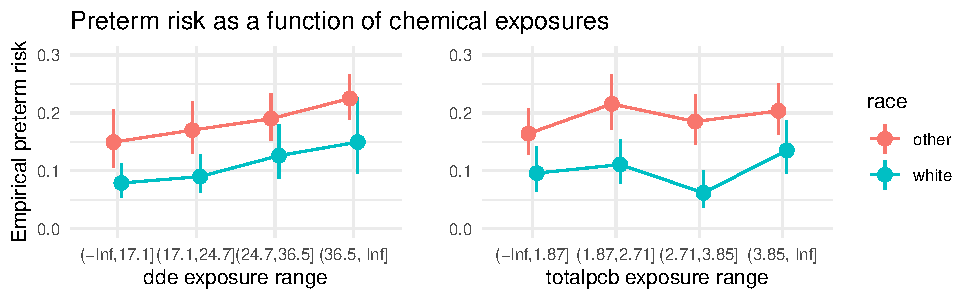
\includegraphics{report_files/figure-latex/marginal effect plot-1.pdf}
\caption{Marginal relationship between empirical preterm risk and
chemical exposures, without controlling for socio-economic and health
variables. The exposure ranges have been defined so that each class
contains 25\% of the observations and vertical lines represent 95\%
confidence intervals for the estimated risk.}
\end{figure}

\hypertarget{missing-values-imputation}{%
\subsection{2.2 Missing Values
Imputation}\label{missing-values-imputation}}

The \(22\%\) missing values in the \emph{score\_*} variables were
imputed under a missing at random assumption using a standard Bayesian
framework. We treated the score variables as independent, identically
distributed Normal random variables and fitted a Bayesian linear model
using the other predictor variables and a non-informative prior. That
is, we regressed the observed values of the \emph{score\_*} variables
onto the other predictor variables and treated missing score values as
model parameters, estimated through their posterior mean.

This approach has two major limitations. First, separating imputation
from model fitting prevents the propagation of imputation uncertainty,
although the Bayesian formulation would allow to combine the two steps
together. Second, our approach assumes that observed variables in the
data set can adequately predict the missing score values, or that data
is missing at random. Even if this were to be the case, the data does
not suggest clear linear relationships between the \emph{score\_*}
variables and other predictors. The potential of more complex non-linear
models for the analysis of this dataset is considered in the Discussion
section.

\hypertarget{logistic-regression-model-for-preterm-outcome.}{%
\subsection{2.3 Logistic regression model for preterm
outcome.}\label{logistic-regression-model-for-preterm-outcome.}}

We model the log odds ratio of preterm birth as a linear function of the
other covariates and perform maximum likelihood estimation. This allows
us to control for the baseline effect of the \emph{race},
\emph{smoking\_status} and \emph{center} factors, and to control for the
linear effect of socio-economic and health-related variables
(\emph{maternal\_age}, \emph{score\_income}, \emph{score\_education},
\emph{score\_occupation}, \emph{cholesterol}, and \emph{triglycerides})
on the log odds ratio. Appart from \emph{dde} and \emph{totalpcb}, no
other variables are incorporated into this base model, and no
interaction terms are considered.

The importance of the \emph{dde} and \emph{totalpcb} variables is
assessed by: (1) testing for individual and joint statistical
significance of the variables; (2) by transforming the associated
\(p\)-values to the more meaningful \(B(p) = -e p \log(p)\) scale; and
(3) by interpreting the estimated effect size. For part (1), individual
statistical significance is based on standard approximate \(t\)-tests
and joint significance is tested with an approximate \(\chi^2\) test.
The rationale for (2) is that \(B(p)\) provides a lower bound on the
Bayes factor comparing the null hypothesis of no effect to the
alternative (over a large nonparametric class of reasonable prior
distributions and when \(p < e^{-1}\); see \citet{Sellke2001}). For
example, a \(p\)-value of \(0.01\) is transformed to
\(B(0.01) \approx 1/8\): if both the null and the alternative hypotheses
are a priori equally likely, then a posteriori the alternative
hypothesis cannot be more than 8 times more likely than the null. Our
interpretation (3) relies on the multiplicative contribution of the
\emph{dde} and \emph{pcb} coefficients on the odds ratio of preterm
birth, as a function of the empirical quantiles of exposure.

\hypertarget{results}{%
\section{3. Results}\label{results}}

Figure 2 below shows the clinically significant estimated effects of the
\emph{dde} and \emph{totalpcb} variables. The estimated odds ratio,
i.e.~the estimated probability of preterm birth to non-preterm birth,
can more than double as exposure to \emph{dde} or \emph{totalpcb} goes
from zero to some of the larger concentration values observed in the
dataset. This is roughly comparable to the marginal effect (which does
not take into account the control variables) shown in the left panel of
Figure 1. Note that the \emph{dde} and \emph{totalpcb} effect estimators
are correlated (\(\hat \rho = -0.29\)), contributing to the rather large
width of the confidence intervals. Furthermore, we warn that the
estimated multiplicative effect in the tail may be unreliable. While we
expect the logistic regression to properly capture overall trends, there
is not reason for it to adequately fit more particular features of the
data.

\begin{figure}

{\centering 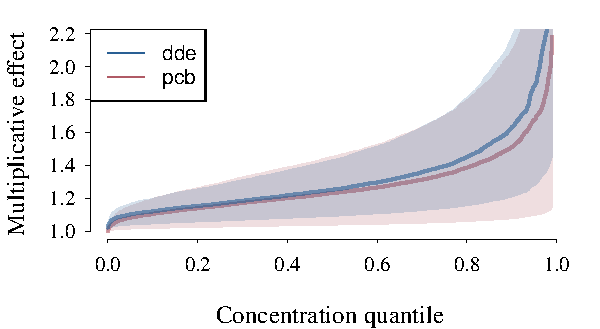
\includegraphics{report_files/figure-latex/unnamed-chunk-3-1} 

}

\caption{Multiplicative effect of dde and totalpcb on the odds ratio of preterm to non-preterm birth, as a function of the empirical dde or pcb concentration quantile. Confidence intervals are represented by shaded regions, and the plot is truncated on the right at the 0.99 quantile.}\label{fig:unnamed-chunk-3}
\end{figure}

Furthermore, the \emph{dde} and \emph{totalpcb} variables have
statistically significant effects: it is unlikely that a trend of this
order would have arised by chance under the logistic model. The
\(p\)-values computed can be interpreted on the \(-e p \log(p)\) scale:
the Bayes factor in favor of a non-null effect could be up to 47 to 1
for the \emph{dde} variable, and up to 5.8 to 1 for the \emph{totalpcb}
variable.

\begin{longtable}[]{@{}rccc@{}}
\toprule
& \emph{dde} & \emph{totalpcb} & jointly\tabularnewline
\midrule
\endhead
\(p\)-value & \(1.2\cdot 10^{-3}\) & \(1.5 \cdot 10^{-2}\) &
\(2.27 \cdot 10^{-5}\)\tabularnewline
\(B(p)\) & 1/47 & 1/5.8 & 1/1514\tabularnewline
\bottomrule
\end{longtable}

The effect of \emph{dde} and \emph{totalpcb} on preterm risk found in
this data, after superficially controlling for confounding factors, is
very concerning. However, we cannot currently single out any of these
two variables as having a distinct effect on preterm birth. The results
should also be considered with care, as we do not expect the logistic
model to correctly capture the data-generating mechanism. Inference
about the ``existence'' of an effect is not meaningful in this context,
and our analysis should be understood as only showcasing a particular
aspect of this data.

\hypertarget{discussion}{%
\section{4. Discussion}\label{discussion}}

We used a logistic regression to estimate the effect of \emph{dde} and
\emph{totalpcb} on preterm risk, controlling for socio-economic and
health-related variables. This allowed us to display a significant
association between presence of these chemicals and preterm risk: higher
concentrations increased the estimated risk of preterm birth.

However, important limitations prevent us from drawing definitive
conclusions from this analysis. In addition to the issues previously
mentioned, our methodological approach could have been improved. First,
it is clear that the logistic model, without any transformation of
variables or interactions, does not correspond to a plausible
data-generating model. In this context, the \(p\)-values and Bayes
factors computed conditionally on null logistic models are not very
meaningful, and a non-parametric bootstrap approach to the computation
of \(p\)-values and confidence intervals would have provided more
adequate quantification of uncertainty. Second, we could consider
non-linear models to better control for the socio-economic and
health-related variables. This is considered in the appendix with a
random forest regression of gestational age, and a heuristic is proposed
to assess variable significance in this context.

\newpage

\hypertarget{appendix}{%
\section{Appendix}\label{appendix}}

\hypertarget{data-visualization}{%
\subsection{Data visualization}\label{data-visualization}}

We plot some aspect of the data below, showcasing the marginal
association between some of the variables and gestational age.

First, we consider the gestational age distribution disaggregated by
race. The left panel below further distinguishes smoking and non-smoking
women, and the right panel shows the gestational age distribution in the
different centers. We notice that non-white women have a much heavier
left tail of gestational age, corresponding to higher preterm risk.
Smoking also seems to affect preterm risk, but to a lesser extent. On
the right, we notice slight heterogeneity between centers, with only a
few of them notably differing from the others (centers 10 and 55).

\begin{center}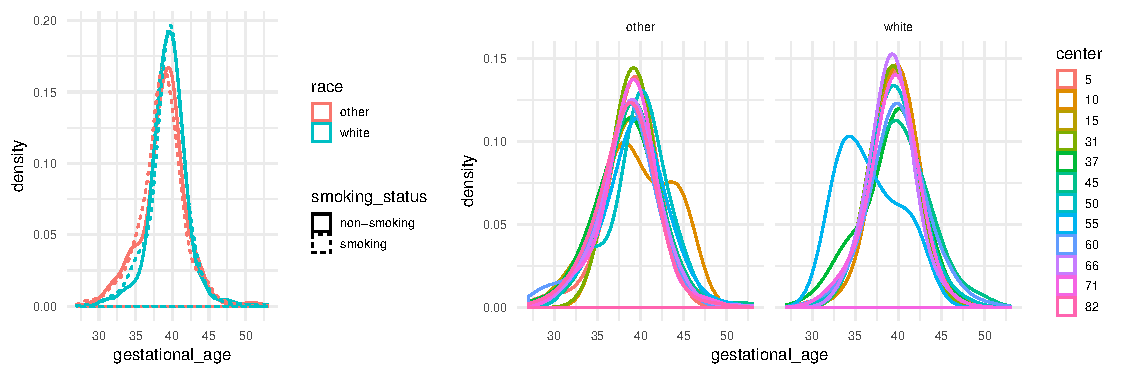
\includegraphics{report_files/figure-latex/unnamed-chunk-5-1} \end{center}

Next, we plot the distribution of chemical concentrations,
disaggregating among women with late preterm ( \(\geq 34\) weeks and
\(< 37\) weeks), very preterm (\(< 34\) weeks) or non-preterm births.
For women with late preterm birth, the chemical concentration
distribution seems heavier on the right. This is not clearly seen for
women with very preterm births, although not seeing an effect here may
be due to the low sample size in this category.

\begin{center}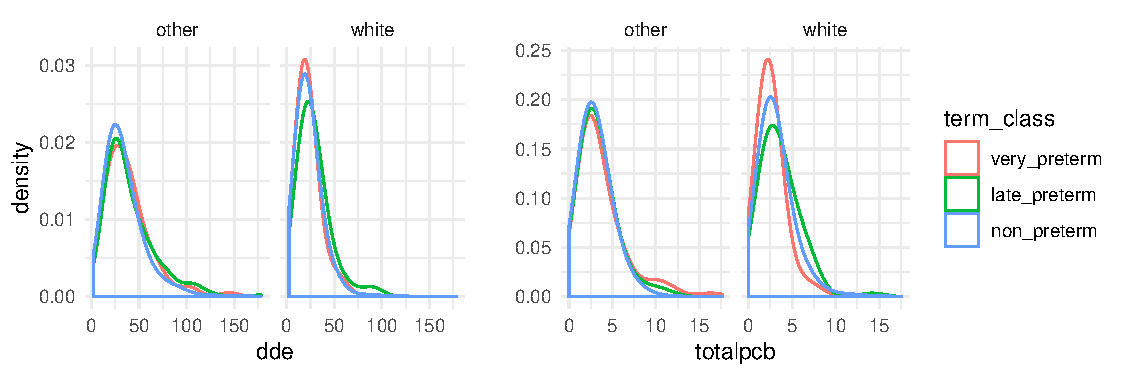
\includegraphics{report_files/figure-latex/unnamed-chunk-6-1} \end{center}

Finally, we reproduce below Figure 1, which shows preterm risk as a
function of range of chemical concentrations, adding to it the empirical
very preterm risks. There is no clear marginal relationship between
chemical concentrations and very preterm risks.

\begin{center}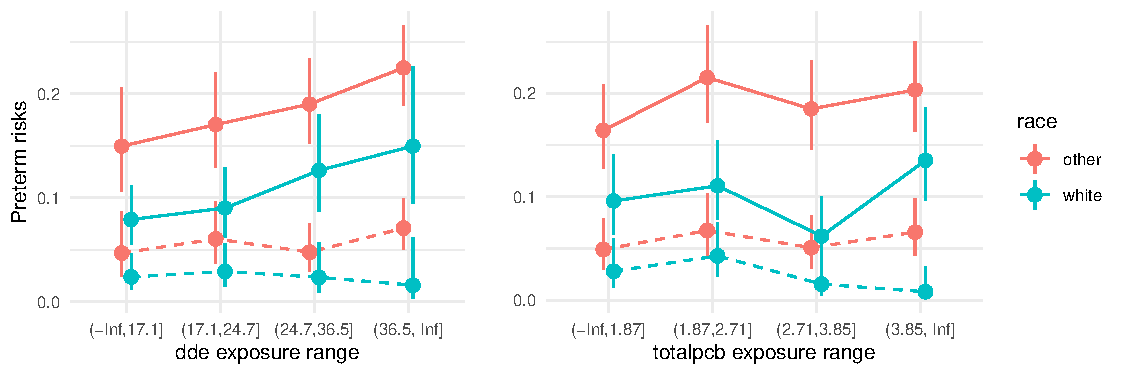
\includegraphics{report_files/figure-latex/unnamed-chunk-7-1} \end{center}

\hypertarget{bayesian-model-averaging}{%
\subsection{Bayesian model averaging}\label{bayesian-model-averaging}}

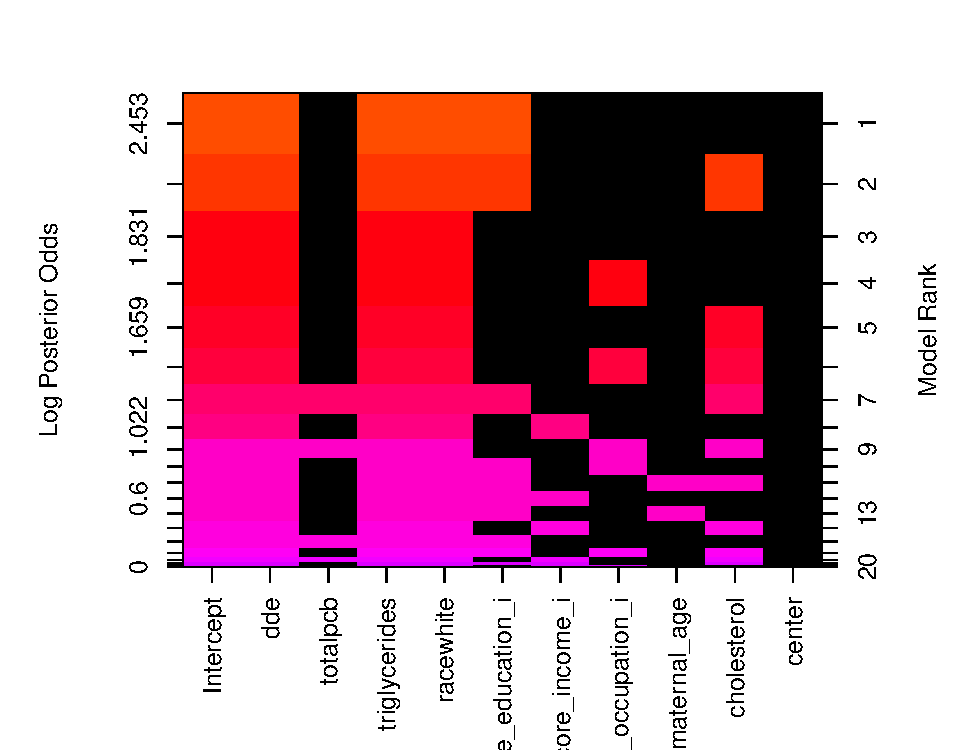
\includegraphics{report_files/figure-latex/unnamed-chunk-8-1.pdf}

Since cases classified as preterm and early preterm comprise relatively
small porportions of the data, and since we reduced the individual PCB
variables into one aggregate totalpcb variable, we check the
significance of these variables through Bayesian Model Averaging (BMA).
This process works by assigning a prior distribution to the set of
possible models, and then uses the observed data set to calculate
posterior probabilities for each of the possible models. One advantage
of this method is that we obtain a posterior probability for each
variable, which serves as a way to quantify undercertainty about each
variable's statistical significance.

Using a uniform prior distribution on the set of models, we conduct BMA
on the models outlined above. The posterior probabilities of each
variable are provided below.

BMA mostly confirms the statstical significances found through logistic
regression, but notably highlights uncertainty about the explanatory
power of PCB in the model. We believe this inconsistency is due to the
low number of preterm and earlypreterm births observed in the dataset,
and note that further study should be done to asses the statistical
significance of PCB.

In comparing results based on different definitions of preterm birth, we
find that it is likely the case that DDE (and to a lesser extent, PCB)
are associated with early birth. However, in the more extreme cases,
where gestational age is less than 34 years, there are likely other
factors not represented in the data that account for this difference.

\hypertarget{non-linear-interactions}{%
\subsection{Non-linear interactions}\label{non-linear-interactions}}

We use a random forest to regress \emph{gestational\_age} onto the other
variables (the same used as in the main analysis). In comparison to the
abysmall predictive accuracy of the logistic regression model (\(85\%\),
which is barely better than a trivial classifier in this context), the
random forest model correctly classifies \(95.5\%\) of the cases over
the training data. While there could be overffiting here, this is
inconsequential in the interpretation of the following analysis.

In order to assess the importance of the dde variable in this context,
we consider the distribution of the random forest predictive accuracy
when \emph{dde} is replaced by white noise. This is plotted below.

\begin{figure}

{\centering 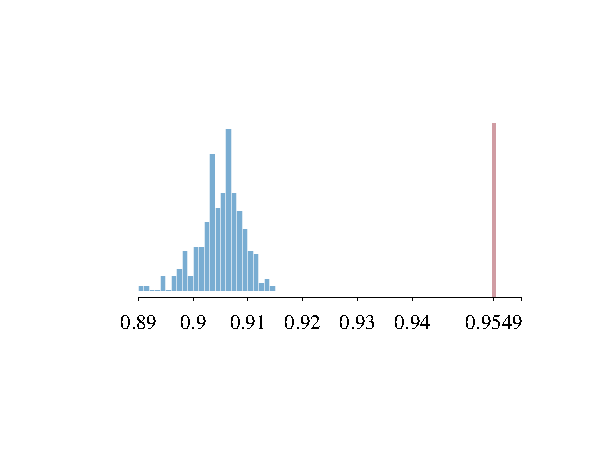
\includegraphics{report_files/figure-latex/unnamed-chunk-10-1} 

}

\caption{Distribution of the random forest predictive accuracy when dde has been replaced by white noise. The predictive accuracy of the random forest model with the dde variable is marked by a red vertical line.}\label{fig:unnamed-chunk-10}
\end{figure}

This shows \emph{dde} has a much more significant effect on predictive
accuracy than a random noise covariate would have, even after
controlling for the other confounding variables. The results obtained in
the main analysis are therefore somewhat robust to the consideration of
non-linear relationships in the data.

The above heuristic is not exactly standard, but it can be interpreted,
for example, in the context of a standard linear model with gaussian
errors. Using the \(R^2\) goodness of fit statistic in this linear model
context, the above procedure is entirely equivalent to a standard
\(F\)-test. For non-linear models, it is not quite as clear wether a
white noise null hypothesis is appropriate. Randomly permuting the dde
values could alternatively provide a distribution for the random noise
covariate. This doesn't noticeably change the results in our case.





\newpage
\singlespacing 
\bibliography{biblio.bib}

\end{document}
